In this appendix we will develop long calculations appeared throughout different chapters.

\subsection[Simplification of the Eq.~{(\ref{eq:vd-result-before-simp})}]
{Simplification of $\expect{\{J_x^2,J_y^2\}+\{J_x,J_y\}^2}$}
\label{ap:loca-simplification}

The expectation value appearing on Equation~{(\ref{eq:vd-result-before-simp})} which we want to simplify has 6 different terms, all with two $J_x$ and another two $J_y$,
\be
  \expect{J_x^2J_y^2} + \expect{J_xJ_yJ_xJ_y} + \expect{J_xJ_y^2J_x}
  + \expect{J_yJ_x^2J_y} + \expect{J_yJ_xJ_yJ_x} + \expect{J_y^2J_x^2}.
\ee
From all those terms the third is somehow referent, since the pure unpolarised Dicke state used as reference is align with the $x$-axis, so $J_x\ket{D_N^{N/2}}_x=0$.

We use the commutation relations of the angular momentum operators $[J_k,J_l]=\epsilon_{klm} iJ_m$ to rearrange all operators,
\begin{subequations}
\begin{align}
  \expect{J_x^2J_y^2} & = i\expect{J_xJ_zJ_y}+\expect{J_xJ_yJ_xJ_y},
  \label{eq:ap-simplification-1} \\
  \expect{J_xJ_yJ_xJ_y} & = i\expect{J_xJ_yJ_z}+\expect{J_xJ_y^2J_x},
  \label{eq:ap-simplification-2} \\
  \expect{J_xJ_y^2J_x} & = \expect{J_xJ_y^2J_x},
  \label{eq:ap-simplification-3} \\
  \expect{J_yJ_x^2J_y} & = i\expect{J_yJ_xJ_z} + \expect{J_yJ_xJ_yJ_x},
  \label{eq:ap-simplification-4} \\
  \expect{J_yJ_xJ_yJ_x} & = -i\expect{J_zJ_yJ_x} + \expect{J_xJ_y^2J_x},
  \label{eq:ap-simplification-5} \\
  \expect{J_y^2J_x^2} & = -i\expect{J_yJ_zJ_x} + \expect{J_yJ_xJ_yJ_x}.
  \label{eq:ap-simplification-6}
\end{align}
\end{subequations}
One may notice that with those relations is enough to see that we have six $\expect{J_xJ_y^2J_x}$, for instance, Equation~{(\ref{eq:ap-simplification-1})} is $i\expect{J_xJ_zJ_y}$ plus Equation~{(\ref{eq:ap-simplification-2})} which at the same time is $i\expect{J_xJ_yJ_z}$ plus Equation~{(\ref{eq:ap-simplification-3})}.
So each equation has at the end one $\expect{J_xJ_y^2J_x}$ plus or minus some expectation value of the product of three operators.

For the three terms operators and again using the commutation relations we can further simplify this expression. Trying to get one $\expect{J_xJ_yJ_z}$ on each term, we obtain the following,
\begin{subequations}
\begin{align}
  i\expect{J_xJ_zJ_y} & = \expect{J_x^2}+i\expect{J_xJ_yJ_z},
  \label{eq:ap-last-terms-1} \\
  2i\expect{J_xJ_yJ_z} & = 2i\expect{J_xJ_yJ_z},
  \label{eq:ap-last-term-2} \\
  i\expect{J_yJ_xJ_z} & = \expect{J_z^2}+i\expect{J_xJ_yJ_z},
  \label{eq:ap-simplification-3} \\
  -i\expect{J_yJ_zJ_x} & = \expect{J_y^2} - \expect{J_z} - i\expect{J_xJ_yJ_z} \\
\begin{split}
  -3i\expect{J_zJ_yJ_x} & = -3\expect{J_x^2} - 3i \expect{J_yJ_zJ_x} \\
  & = -3\expect{J_x^2} + 3 \expect{J_y^2} - 3i\expect{J_yJ_xJ_z} \\,
  & = -3\expect{J_x^2} + 3 \expect{J_y^2} - 3\expect{J_z^2}
   - 3i \expect{J_xJ_yJ_z}.
  \label{eq:ap-simplification-4}
\end{split}
\end{align}
\end{subequations}
Now if we sum it all, note that the all 3 operators terms simplify, and if we take into account $6\expect{J_xJ_y^2J_x}$ the resulting expression is the following,
\be
   4\expect{J_y^2} - 3 \expect{J_z^2} - 2\expect{J_x^2} + 6\expect{J_xJ_y^2J_x}
\ee

\subsection{Legendre transform}

The Legendre transform of a convex function, say $f:x \rightarrow f(x)$, is defined as the maximum distance between the function the line $rx$ and $f(x)$ at same $x$.
In can be written as follows,
\be
  \hat{f}(r):=\max_{x}\{rx-f(x)\},
\ee
where $\hat{f}(r)$ represents the transformed function.
A geometric representation of the transform is given on the Figure~\ref{fig:lt-geometric-legendre}.

\begin{figure}
  \centering
  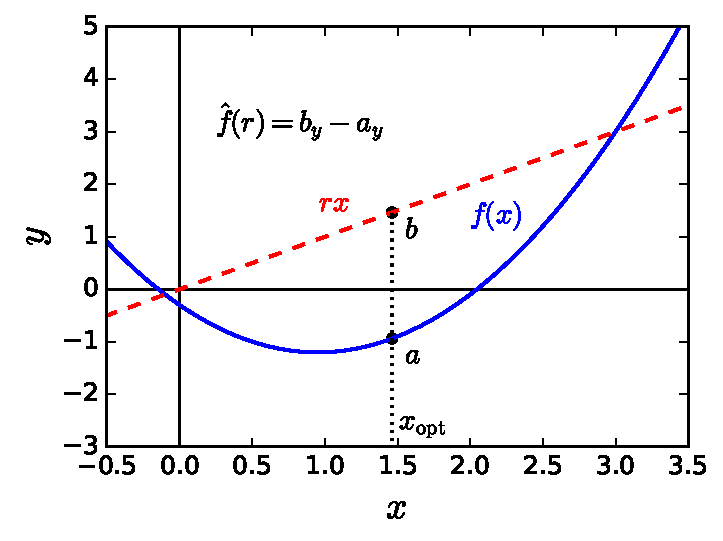
\includegraphics[scale=.65]{img/plots/LT_legendre.pdf}
  \caption{Graphical representation of the Legendre transform. (blue-line) Convex function, $f(x)=x^2-1.9x-0.3$, to be transformed. (red-dashed) Constant slope line passing by the coordinate system origin, $rx$. The Legendre transform is the maximal difference between $rx$ and $f(x)$ at the same $x$. In this case, the vertical distance between $a$ and $b$.}
  \label{fig:lt-geometric-legendre}
\end{figure}

The inverse transformation is simply obtained by applying again the same technique.
One fully recovers the
\be
  f(x) = \max_{r}\{rx-\hat{f}(r)\}.
\ee

Let us develop the example shown in the Figure~\ref{fig:lt-geometric-legendre}, where the function is $f(x)=x^2-1.9x-0.3$.
In this case the problem is well defined on the complete real axis.
Now, one has to find the maximum of $g(r,x)=rx-f(x)$ for all $\forall r$.
This maximum is easily obtained in this particular case with usual techniques.
On has to solve for x the following equation $\partial_x g(r,x) = 0$. Thus, the maximum is at $x_{\text{opt}} = \frac{r+1.9}{2}$ and hence, the Legendre transform is the following,
\be
  \hat{f}(r) = \frac{r^2}{4}+0.95r+1.2025.
\ee
If one applies again the transformation the resulting function is again the original one.
